\documentclass[a4paper,11pt]{article}
\usepackage{array}
\usepackage{tabularx}
\usepackage{booktabs}
\usepackage{graphicx}
\newcommand{\ra}[1]{\renewcommand{\arraystretch}{#1}}
% define the title
\title{Hand-in 1}
\author{\textbf{\textit{Group 4 - SimbasSlaver}}\\
  Claus Lindquist Henriksen \textit{(clih@itu.dk)}\\
  Michael Søby Andersen \textit{(msoa@itu.dk)}\\
  Mikkel Stolborg \textit{(msto@itu.dk)}\\
  Rasmus Agnvig \textit{(raag@itu.dk)}\\
  Hans Pagh - \textit{(hkkp@itu.dk)}
}
\begin{document}
% generates the title
\maketitle
\newpage
% insert the table of contents
\tableofcontents
\newpage
\section{E-R diagrams}
\subsection{Visio ER diagram}
\begin{figure}[h!]
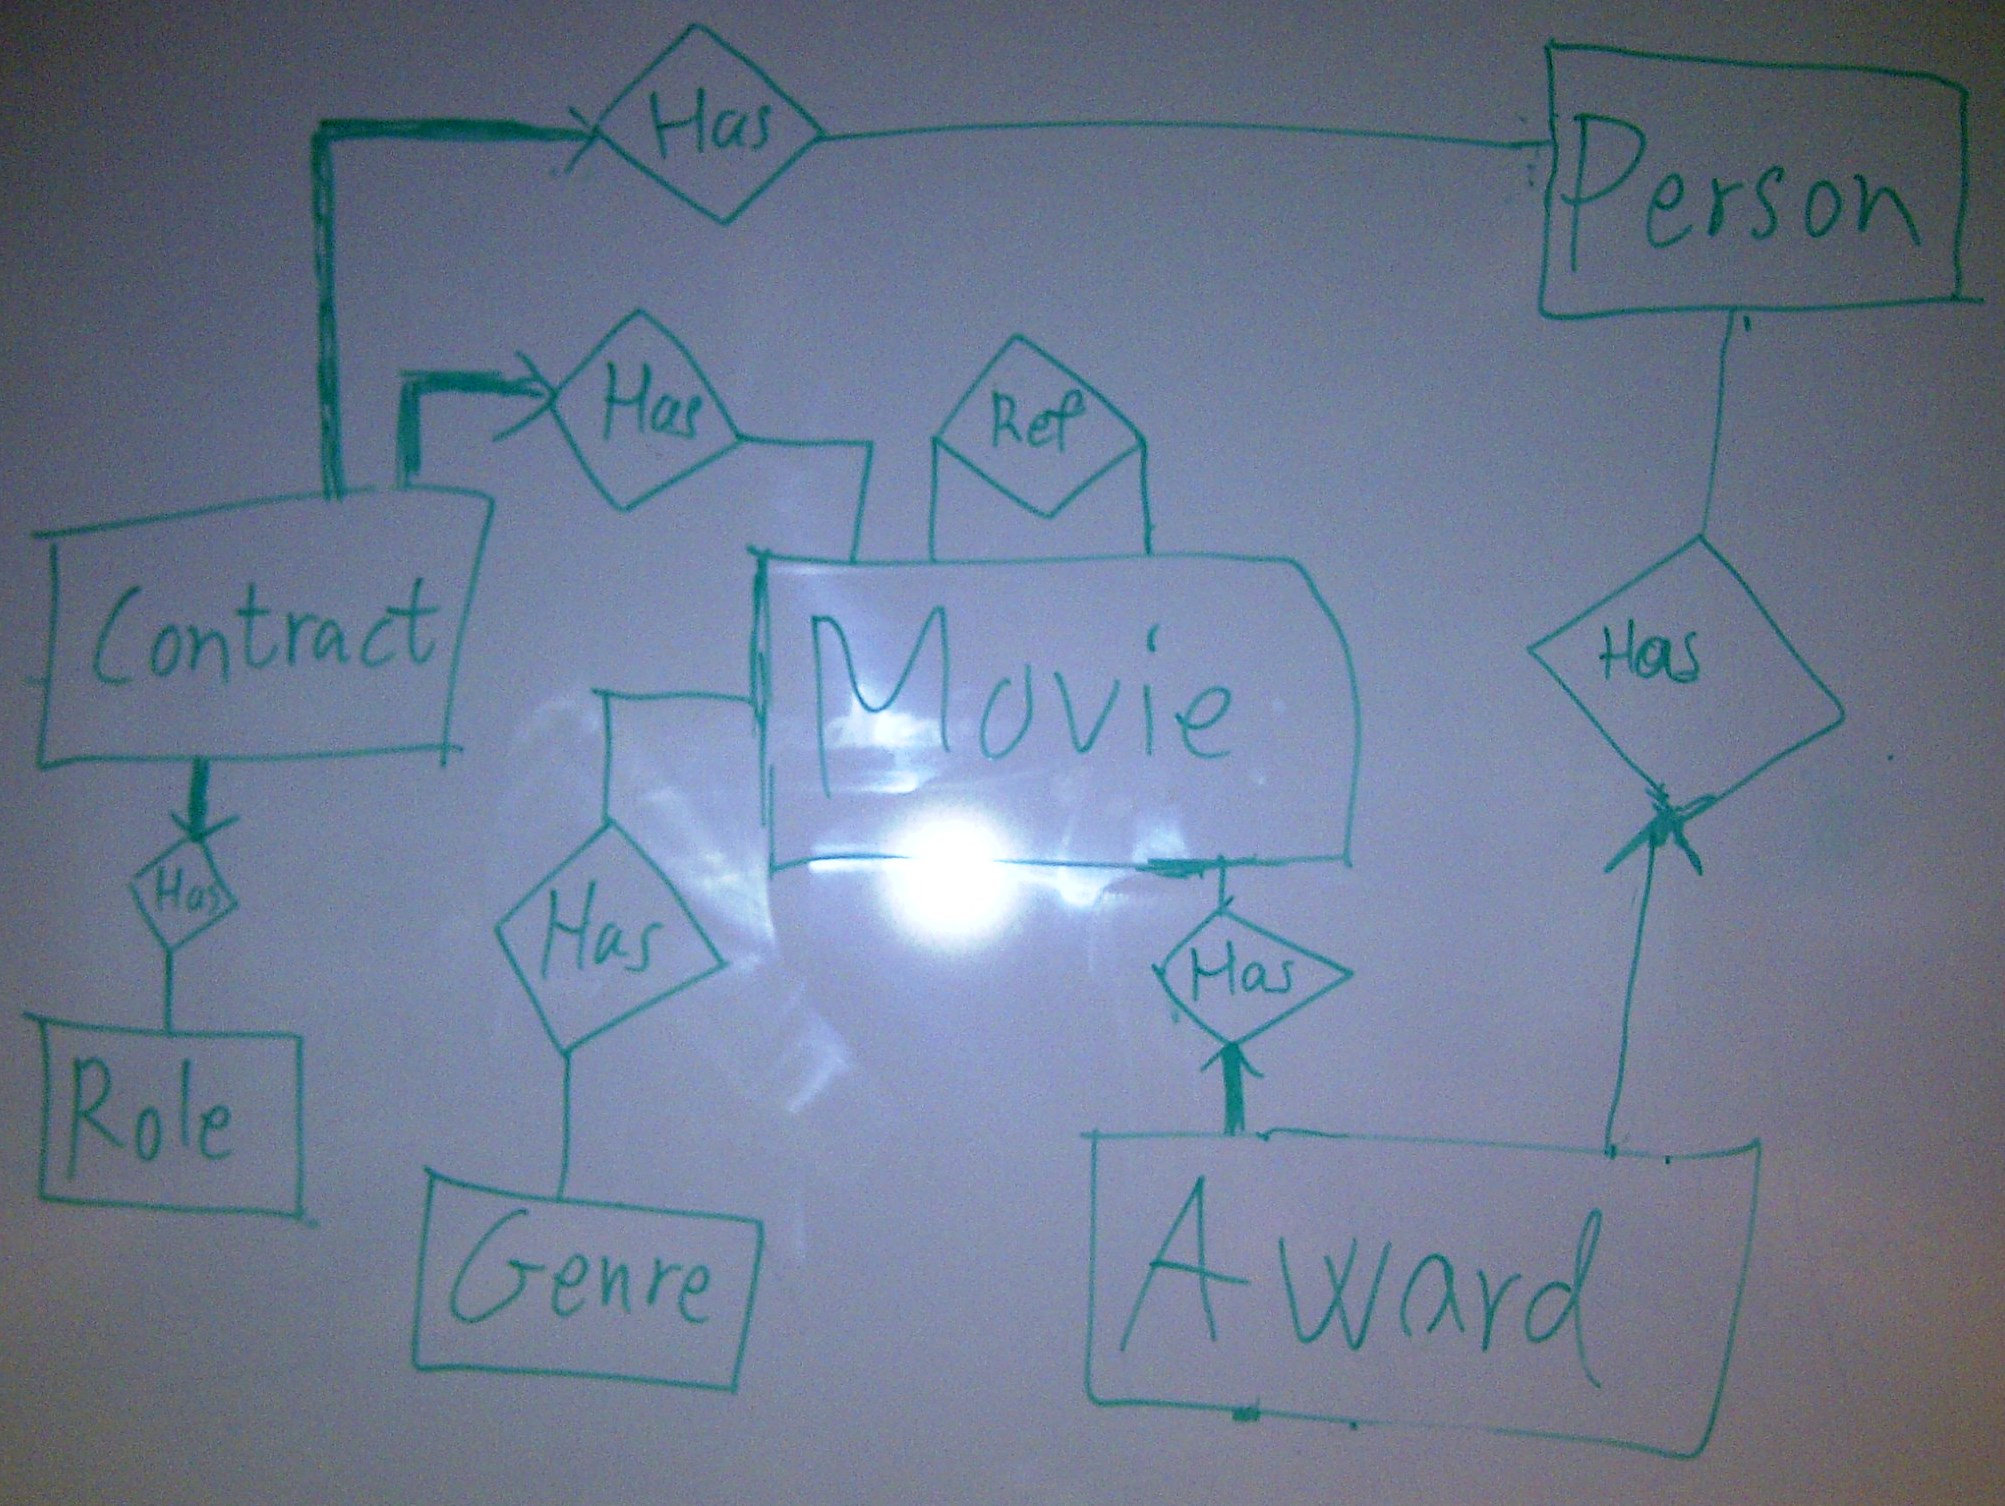
\includegraphics[width=\textwidth,natwidth=825,natheight=699]{illustrations/ER.jpg}
  \caption{Visio ER diagram}
\end{figure}
\subsection{Workbench RG diagram}
\begin{figure}[h!]
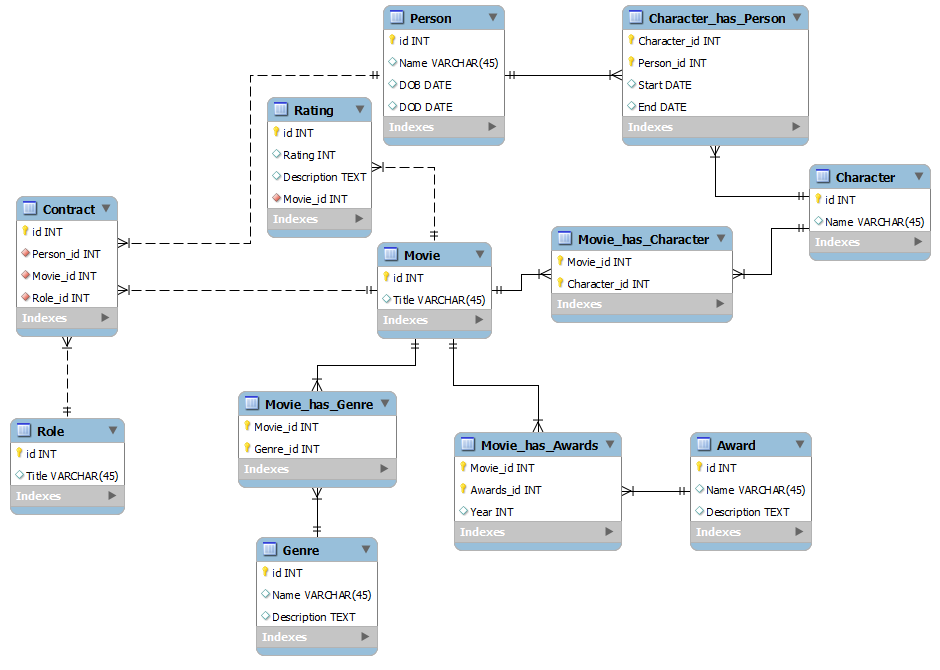
\includegraphics[width=\textwidth,natwidth=940,natheight=670]{illustrations/RG.png}
  \caption{Workbench RG diagram}
\end{figure}
\subsection{Changes since hand-in 1}
We have changed our model since our first hand-in. In our previous model an actor was unable to receive an award.

\newpage

\section{MySQL Schema}
\begin{lstlisting}[language=sql]
SET @OLD_UNIQUE_CHECKS=@@UNIQUE_CHECKS, UNIQUE_CHECKS=0;
SET @OLD_FOREIGN_KEY_CHECKS=@@FOREIGN_KEY_CHECKS, FOREIGN_KEY_CHECKS=0;
SET @OLD_SQL_MODE=@@SQL_MODE, SQL_MODE='TRADITIONAL,ALLOW_INVALID_DATES';

CREATE SCHEMA IF NOT EXISTS `mydb` DEFAULT CHARACTER SET latin1 COLLATE latin1_swedish_ci ;
USE `mydb` ;

-- -----------------------------------------------------
-- Table `mydb`.`Person`
-- -----------------------------------------------------
CREATE  TABLE IF NOT EXISTS `mydb`.`Person` (
  `id` INT NOT NULL AUTO_INCREMENT ,
  `Name` VARCHAR(45) NULL ,
  `DOB` DATE NULL ,
  `DOD` DATE NULL ,
  PRIMARY KEY (`id`) )
ENGINE = InnoDB;


-- -----------------------------------------------------
-- Table `mydb`.`Movie`
-- -----------------------------------------------------
CREATE  TABLE IF NOT EXISTS `mydb`.`Movie` (
  `id` INT NOT NULL ,
  `Title` VARCHAR(45) NULL ,
  PRIMARY KEY (`id`) )
ENGINE = InnoDB;


-- -----------------------------------------------------
-- Table `mydb`.`Genre`
-- -----------------------------------------------------
CREATE  TABLE IF NOT EXISTS `mydb`.`Genre` (
  `id` INT NOT NULL ,
  `Name` VARCHAR(45) NULL ,
  `Description` TEXT NULL ,
  PRIMARY KEY (`id`) )
ENGINE = InnoDB;


-- -----------------------------------------------------
-- Table `mydb`.`Award`
-- -----------------------------------------------------
CREATE  TABLE IF NOT EXISTS `mydb`.`Award` (
  `id` INT NOT NULL ,
  `Name` VARCHAR(45) NULL ,
  `Description` TEXT NULL ,
  PRIMARY KEY (`id`) )
ENGINE = InnoDB;


-- -----------------------------------------------------
-- Table `mydb`.`Role`
-- -----------------------------------------------------
CREATE  TABLE IF NOT EXISTS `mydb`.`Role` (
  `id` INT NOT NULL ,
  `Title` VARCHAR(45) NULL ,
  PRIMARY KEY (`id`) )
ENGINE = InnoDB;


-- -----------------------------------------------------
-- Table `mydb`.`Contract`
-- -----------------------------------------------------
CREATE  TABLE IF NOT EXISTS `mydb`.`Contract` (
  `id` INT NOT NULL ,
  `Person_id` INT NOT NULL ,
  `Movie_id` INT NOT NULL ,
  `Role_id` INT NOT NULL ,
  PRIMARY KEY (`id`) ,
  INDEX `fk_Contract_Person1_idx` (`Person_id` ASC) ,
  INDEX `fk_Contract_Movie1_idx` (`Movie_id` ASC) ,
  INDEX `fk_Contract_Role1_idx` (`Role_id` ASC) ,
  CONSTRAINT `fk_Contract_Person1`
    FOREIGN KEY (`Person_id` )
    REFERENCES `mydb`.`Person` (`id` )
    ON DELETE NO ACTION
    ON UPDATE NO ACTION,
  CONSTRAINT `fk_Contract_Movie1`
    FOREIGN KEY (`Movie_id` )
    REFERENCES `mydb`.`Movie` (`id` )
    ON DELETE NO ACTION
    ON UPDATE NO ACTION,
  CONSTRAINT `fk_Contract_Role1`
    FOREIGN KEY (`Role_id` )
    REFERENCES `mydb`.`Role` (`id` )
    ON DELETE NO ACTION
    ON UPDATE NO ACTION)
ENGINE = InnoDB;


-- -----------------------------------------------------
-- Table `mydb`.`Rating`
-- -----------------------------------------------------
CREATE  TABLE IF NOT EXISTS `mydb`.`Rating` (
  `id` INT NOT NULL ,
  `Rating` INT NULL ,
  `Description` TEXT NULL ,
  `Movie_id` INT NOT NULL ,
  PRIMARY KEY (`id`) ,
  INDEX `fk_Rating_Movie1_idx` (`Movie_id` ASC) ,
  CONSTRAINT `fk_Rating_Movie1`
    FOREIGN KEY (`Movie_id` )
    REFERENCES `mydb`.`Movie` (`id` )
    ON DELETE NO ACTION
    ON UPDATE NO ACTION)
ENGINE = InnoDB;


-- -----------------------------------------------------
-- Table `mydb`.`Movie_has_Awards`
-- -----------------------------------------------------
CREATE  TABLE IF NOT EXISTS `mydb`.`Movie_has_Awards` (
  `Movie_id` INT NOT NULL ,
  `Awards_id` INT NOT NULL ,
  `Year` INT NULL ,
  PRIMARY KEY (`Movie_id`, `Awards_id`) ,
  INDEX `fk_Movie_has_Awards_Awards1_idx` (`Awards_id` ASC) ,
  INDEX `fk_Movie_has_Awards_Movie1_idx` (`Movie_id` ASC) ,
  CONSTRAINT `fk_Movie_has_Awards_Movie1`
    FOREIGN KEY (`Movie_id` )
    REFERENCES `mydb`.`Movie` (`id` )
    ON DELETE NO ACTION
    ON UPDATE NO ACTION,
  CONSTRAINT `fk_Movie_has_Awards_Awards1`
    FOREIGN KEY (`Awards_id` )
    REFERENCES `mydb`.`Award` (`id` )
    ON DELETE NO ACTION
    ON UPDATE NO ACTION)
ENGINE = InnoDB;


-- -----------------------------------------------------
-- Table `mydb`.`Character`
-- -----------------------------------------------------
CREATE  TABLE IF NOT EXISTS `mydb`.`Character` (
  `id` INT NOT NULL ,
  `Movie_id` INT NOT NULL ,
  `Name` VARCHAR(45) NULL ,
  INDEX `fk_Characters_Movie1_idx` (`Movie_id` ASC) ,
  PRIMARY KEY (`id`) ,
  CONSTRAINT `fk_Characters_Movie1`
    FOREIGN KEY (`Movie_id` )
    REFERENCES `mydb`.`Movie` (`id` )
    ON DELETE NO ACTION
    ON UPDATE NO ACTION)
ENGINE = InnoDB;


-- -----------------------------------------------------
-- Table `mydb`.`Character_has_Person`
-- -----------------------------------------------------
CREATE  TABLE IF NOT EXISTS `mydb`.`Character_has_Person` (
  `Character_id` INT NOT NULL ,
  `Person_id` INT NOT NULL ,
  `Start` DATE NULL ,
  `End` DATE NULL ,
  PRIMARY KEY (`Character_id`, `Person_id`) ,
  INDEX `fk_Character_has_Person_Person1_idx` (`Person_id` ASC) ,
  INDEX `fk_Character_has_Person_Character1_idx` (`Character_id` ASC) ,
  CONSTRAINT `fk_Character_has_Person_Character1`
    FOREIGN KEY (`Character_id` )
    REFERENCES `mydb`.`Character` (`id` )
    ON DELETE NO ACTION
    ON UPDATE NO ACTION,
  CONSTRAINT `fk_Character_has_Person_Person1`
    FOREIGN KEY (`Person_id` )
    REFERENCES `mydb`.`Person` (`id` )
    ON DELETE NO ACTION
    ON UPDATE NO ACTION)
ENGINE = InnoDB;


-- -----------------------------------------------------
-- Table `mydb`.`Movie_has_Genre`
-- -----------------------------------------------------
CREATE  TABLE IF NOT EXISTS `mydb`.`Movie_has_Genre` (
  `Movie_id` INT NOT NULL ,
  `Genre_id` INT NOT NULL ,
  PRIMARY KEY (`Movie_id`, `Genre_id`) ,
  INDEX `fk_Movie_has_Genre_Genre1_idx` (`Genre_id` ASC) ,
  INDEX `fk_Movie_has_Genre_Movie1_idx` (`Movie_id` ASC) ,
  CONSTRAINT `fk_Movie_has_Genre_Movie1`
    FOREIGN KEY (`Movie_id` )
    REFERENCES `mydb`.`Movie` (`id` )
    ON DELETE NO ACTION
    ON UPDATE NO ACTION,
  CONSTRAINT `fk_Movie_has_Genre_Genre1`
    FOREIGN KEY (`Genre_id` )
    REFERENCES `mydb`.`Genre` (`id` )
    ON DELETE NO ACTION
    ON UPDATE NO ACTION)
ENGINE = InnoDB;



SET SQL_MODE=@OLD_SQL_MODE;
SET FOREIGN_KEY_CHECKS=@OLD_FOREIGN_KEY_CHECKS;
SET UNIQUE_CHECKS=@OLD_UNIQUE_CHECKS;
\end{lstlisting}
\newpage
\section{Analysis}
While going through our E/R model, we searched for FD to make sure that our model was in normal form.
  We have found the following functional dependencies:
  \begin{itemize}
    \item Rating: Movie\_id, Source
    \item Contract: Person\_id, Movie\_id, Role\_id
    \item Award: Award\_year, Award\_name
  \end{itemize}
  We have considered the following scenerios, where one might doubt that our implementations is in normal form: \\
  \subsection{Role}
    \begin{itemize}
      \qaitem {Isnt there a FD between a Person\_id and a Role\_id to Movie\_id in the contract table?}
              {We assume that a person can play more than one role per movie.}
    \end{itemize}
  \subsection{Character}
    \begin{itemize}
      \qaitem {Isnt there a FD between a character and a movie}
              {We assume that a character can apaier in more than once in a movie.}
      \qaitem {Isnt there a FD between a person and a character}
              {More than one person can play one character in movie.}
    \end{itemize}
  \subsection{Rating}
    \begin{itemize}
      \qaitem {Isnt there a FD between Moive and source to rating}
              {Yes. We assume that one source can only rate a movie once , else the rating is just editted}
    \end{itemize}
    All of the IDs in our entities are functional dependencies, but they are
    not worth mentioning.
    We have chosen to use IDs as primary keys on most of our entities. This
    makes our implementation very tight and aside from the IDs themselves, we
    do not have many functional dependencies and consider the model to be in normal form.
\newpage

\end{document}
